\documentclass[12pt]{article} %\documentclass[12pt, twocolumn]{article}
\usepackage[left=2.5cm,right=2.5cm,top=2.5cm,bottom=2.5cm]{geometry}
\usepackage{amsmath}
\DeclareMathOperator{\trace}{trace}
\usepackage{graphicx}
\usepackage[font=small,labelfont=bf]{caption}
\usepackage{fancybox}
\usepackage{array}
\usepackage{multirow}
\usepackage[numbers,square,sort]{natbib}
\usepackage[resetlabels]{multibib}
\usepackage{hyperref}
\usepackage{comment}
\usepackage{makeidx}
\usepackage{amsfonts}
\usepackage{amssymb}
\usepackage{blindtext}
\usepackage{multicol}
\usepackage{enumitem}
\usepackage[mathscr]{euscript}
\setlength{\columnsep}{1cm}
\usepackage{xepersian}
\usepackage[mathscr]{euscript}
\settextfont[Scale=1.2]{XB Niloofar}
\renewcommand{\labelenumii}{\arabic{enumi}.\arabic{enumii}}
\renewcommand{\labelenumiii}{\arabic{enumi}.\arabic{enumii}.\arabic{enumiii}}
\renewcommand{\labelenumiv}{\arabic{enumi}.\arabic{enumii}.\arabic{enumiii}.\arabic{enumiv}}

% Begin Narges's part__________________________________________________________

\title{الگوریتم های تصادفی لاس وگاس در مسائل اجماع توزیع شده}
\author{نرگس قانعی-610399155\\آران باطنی-610399105\\فاطمه رشیدی-610399131}
\date{تیر 1401}

\begin{document}
	\maketitle

	\textbf{چکیده- ما مشکلات اجماع توزیع شده را از دیدگاه الگوریتم های احتمالی در نظر می گیریم
    به خصوص،
    ما یک مرور کلی در مورد برخی از مشکلات خاص ارائه می دهیم
    که در آن
    تصادفی سازی در دستیابی به اجماع بین عوامل متعدد حیاتی است.
    علاوه بر این، ما نشان می دهیم که الگوریتم های تصادفی شده 
    که در این تنظیمات استفاده می شود به اصطلاح الگوریتم های تصادفی لاس وگاس هستند.
     (به عنوان مثال \cite{bib24}).
     این کلاس با نوع مونت کارلو که اخیرا 
     با موفقیت برای مسائل
     مختلف محاسباتی دشوار سیستم ها و کنترل استفاده می شود متفاوت است.
    بنابراین هدف این مقاله این است که
    ارتباط بین مسائل مختلف اجماع توزیع شده 
    و الگوریتم های تصادفی برای سیستم ها و کنترل را نشان بدهد.}

	\tableofcontents
	\newpage

	\section{مقدمه}
	در سال های اخیر، اجماع، توافق، و
	مسائل انبوه توجه زیادی را در سیستم ها و جامعه کنترل به خود جلب کرده است.
	کنترل رویکردهای نظری
	ثابت کرده اند که در تجزیه و تحلیل توزیع شده
	سیستم هایی برای مشخصاتی مانند ثبات و توافق مفید هستند.
	منابع اخیر شامل \cite{bib03}،\cite{bib04}،\cite{bib06}، \cite{bib07}، \cite{bib10}، \cite{bib12}، \cite{bib16}،
	\cite{bib18}، \cite{bib20}، \cite{bib21}، \cite{bib25}،\cite{bib27}است.
 برای جزئیات بیشتر به \cite{bib05} مراجعه می کنیم
	که خلاصه ای از توسعه چنین مسائلی همراه با برخی از نتایج جدید می دهد
	و به ویژه
	شماره \cite{bib01} که تحقیقات جاری در مورد این موضوع را شرح می دهد.
	\par
	به طور خاص، ما میانگین مسائل اجماع را در نظر می گیریم که می توان آنها را به شرح زیر توصیف کرد:
	مجموعه ای از N عواملی که دارای مقادیر عددی هستند وجود دارد
	و ارزش هایشان را به همسایگان خود به شیوه ای تکراری منتقل می کنند.
	هدف این است
	که همه عوامل در نهایت به یک مقدار مشترک برسند که این
	میانگین مقادیر اولیه همه عوامل است.
	چنین مسائلی
	در کاربردهای مرتبط با هماهنگی چند وسیله نقلیه،
	تعادل بار و شبکه های حسگر ایجاد می شود.
	\par
	هدف این مقاله ارائه میانگین مسائل اجماع از نقطه نظر یکپارچه الگوریتم های احتمالی و لاس وگاس می باشد
	اخیراً در زمینه
	سیستم‌ها و کنترل، تکنیک‌های مبتنی بر الگوریتم‌های تصادفی توسعه یافته‌اند (به عنوان مثال، \cite{bib23}، \cite{bib26} را ببینید).
	با این حال،
	خواهیم دید که چگونه کلاس های الگوریتم ها وجود دارد و
	در اجماع مسائل متفاوت عمل می کنند.
	با توجه
	به یک تعریف رسمی مورد استفاده در علوم کامپیوتر \cite{bib17}، یک
	الگوریتم تصادفی الگوریتمی است که در طول اجرای آن برای ایجاد نتیجه انتخاب هایی تصادفی می سازد.
	این دلالت می کند که
	که حتی برای یک ورودی، الگوریتم ممکن است نتایج متفاوت در اجراهای مختلف تولید کند
	و علاوه بر آن نتایج
	حتی ممکن است نادرست باشد.
	\par
	به طور خاص، در این مقاله، ما قصد داریم دو مورد را روشن کنیم
	نکته ها:
	یکی از آنها معرفی الگوریتم‌های تصادفی‌سازی‌شده است که در چندین مورد متفاوت از مسائل اجماع متوسط ​​ظاهر می‌شوند.
	چنین تکنیک هایی نشان داده شده است که مفید هستند و می توانند حیاتی باشند.
	در واقع، در برخی موارد، نتایج حتی قوی تری وجود دارد که نشان می دهد هیچ روش قطعی ای نمی تواند به طور کارآمد به دست آید.
	اجماع \cite{bib09}، \cite{bib17}.
	دیگری نشان دادن تفاوت در
	کلاس های الگوریتم هایی که در مسائل اجماع ظاهر می شوند
	و آنهایی که در رویکرد احتمالی در کنترل هستند است.
	در پایان، ما یک نمای کلی در مورد رویکرد احتمالی در کنترل ارائه می دهیم
	و ببینید که الگوریتم های اصلی از نوع مونت کارلو وجود دارند.
	سپس، نشان می‌دهیم که الگوریتم‌های موجود در
	اجماع متوسط ​​متعلق به الگوریتم های نوع کلاس لاس وگاس است.
	این کلاس اخیرا برای مسائل مربوط به سیستم ها و کنترل  مورد سوء استفاده قرار گرفته است.\cite{bib11}، \cite{bib24}.
	\par
	مقاله بصورت زیر مرتب شده است:
	در بخش دوم، ما
	یک مسئله تحلیل استحکام کلی ارائه می دهیم.
	در بخش سوم، الگوریتم های تصادفی از نوع مونت کارلو برای
	چنین مسائلی مورد بحث قرار می گیرد.
	در بخش چهارم، مقدمه ای بر الگوریتم های لاس وگاس ارائه می دهیم.
	در بخش پنچم،
	سه مورد از مسائل اجماع متوسط ​​را مورد بحث قرار داده واهمیت تکنیک های احتمالی را نشان می دهیم.
	در بخش ششم مقاله نتیجه می گیریم.
	
	\section{رویکرد احتمالی به سیستم های نامشخص}
	در دهه گذشته روشهای احتمالاتی برای سیستمها
	و کنترل به طور قابل توجهی پیشرفت کرده است.
	این تحقیق و 
	همچنین نتایج نشان می دهد که بسیاری از 
	مسائلی که به طور طبیعی در کنترل ایجاد می شوند از نظر محاسباتی دشوار هستند.
	چنین مسائلی
	در مناطقی از جمله سیستم های نامشخص و ترکیبی یافت می شود.
	این
	توسعه و کاربرد تکنیک های احتمالی برای
	مسائل کنترل تجزیه و تحلیل و سنتز ثابت شده است که در الگوریتم های  محاسباتی موثر است.
	برای
	یک حساب دقیق در مورد این موضوع, ما به  \cite{bib23} و\cite{bib26} مراجعه می کنیم.
	\par
	در این بخش یک مسئله ی تجزیه و تحلیل استحکام را معرفی می کنیم که عدم قطعیت های مختلف را در آن می توان نشان داد.
	یک سیستم حاوی اجزای نامشخص داده شده, هدف
	تجزیه و تحلیل استحکام این است که بفهمد کنترل خاص
	خواص  را برای همه ی عدم قطعیت ها می دارد یا خیر.
	این مسئله ی کلی
	می تواند به صورت زیر فرموله شود.
	\par
	ما ابتدا فرض می کنیم که عدم اطمینان در سیستم  توسط یک ماتریس حقیقی / موهومی 
	$\Delta$ 
	نشان داده شده است
	نشان داده شده  و $\Delta$ 
	متعلق به یک مجموعه محدود
	$\mathscr{B}$.
	از سوی دیگر
	ویژگی سیستم با تابع عملکرد 
	$J : \mathscr{B} \rightarrow \mathbb{R}$
	اندازه گیری می شود.
	تابع $J$
	فرض می شود تابعی قابل اندازه گیری است.
	یک مسئله ی تجزیه و تحلیل استحکام کلی این است که بررسی کنید
	که آیا یک سطح عملکرد خاص $\gamma$
	برای همه عدم قطعیت های ممکن
	$\Delta \in \mathscr{B}$
	تضمین شده است یا خیر.
	به عبارت دیگر ما علاقه مند هستیم که پیدا کنیم که آیا
	\begin{equation}
		\label{eqn:(1)}
		J(\Delta ) \leqslant \gamma \textrm{ برای هر } \Delta \in \mathscr{B}
	\end{equation}
	\par
	اگر عدم اطمینان
	$\Delta$
	از نوع عمومی است، از نظر پیچیدگی محاسباتی موانعی برای حل این مسئله وجود دارد
	ما یک رویکرد احتمالی را دنبال می کنیم و معنی استحکام را از معنای قطعی  تغییر می دهیم
	همانطور که در \ref{eqn:(1)} اتفاق افتاده است.
	\par
	در رویکرد احتمالاتی فرض می کنیم که ماتریس عدم قطعیت
	$\Delta \in \mathscr{B}$ 
	یک ماتریس تصادفی است;
	اینجا متغیرهای تصادفی
	با حروف پررنگ نشان داده می شوند.
	اجازه دهید
	$Prob_{\Delta}(.)$
	اندازه گیری احتمال مربوطه مربوط به
	$\Delta$
	باشد.
	\par
	ما دو معیار عملکرد خاص را با استفاده از
	$J(\Delta )$
	در نظر میگیریم.
	اولین مورد عملکرد بدترین حالت است که به صورت زیر تعریف میشود:
	\begin{equation} 	
	   J_{max}:= \sup_{\Delta \in \mathscr{B} }J(\Delta ) 
   \end{equation}
   دیگری عملکرد متوسط است
   \begin{equation*} 	
	   J_{ave}:= E_{\Delta}(J(\Delta )) 
   \end{equation*}
   به طوری که 
   $E_{\Delta}(J(\Delta ))$
   مقدار مورد انتظار تابع عملکرد را با توجه به مجموعه عدم قطعیت
   $\mathscr{B}$
   نشان می دهد.
   \par
	در این تنظیمات مشکل تصمیم گیری به یک وضعیت اشاره دارد
	که پاسخ به یک نمونه بله یا خیر است.
	اینجا,
	ما دو مسئله ی تصمیم گیری نامشخص را برطرف می کنیم:
	برای یک سطح عملکرد
	$\gamma > 0$
	چک کنید که آیا
	$J_{max} \leq \gamma $ و $J_{ave} \leq \gamma$.
	ما بعد نشان می دهیم که این مسائل را می توان در معنای احتمالی به طور  موثر حل کرد.
	یک تابع عملکردی که معمولا در تجزیه و تحلیل استحکام استفاده می شود
	$H^{\infty }$
	که نورم یک سیستم حلقه بسته است.
	در
	این مورد, اجازه دهید تابع
	$J(\Delta)$
	نورم سیستم باشد که
	از اختلال تا خروجی کنترل شده است.
	بسته به
	معیار علاقه, ما ممکن است کار با
	عملکرد بدترین حالت یا عملکرد متوسط را انتخاب کنیم.

   \section{الگوریتم های تصادفی مونت کارلو}
	اکنون الگوریتم های تصادفی مونت کارلو را معرفی می کنیم.
	بیشترین نتایج احتمالی حاصل از سیستم ها و کنترل
	بر اساس این نوع الگوریتم ها هستند.
	بعدا خواهیم دید که
	این کلاس متفاوت از آنکه در مسائل اجماع است ظاهر می شود. تعریف به شرح زیر است \cite{bib17}.
	\par
	تعریف 1: الگوریتم تصادفی مونت کارلو
	یک الگوریتم تصادفی است که ممکن است یک نتیجه ای که نادرست است (به معنای قطعی) تولید کند
	 اما احتمال چنین نتیجه ی نادرستی محدود است.
	\par
	به طور کلی, برای MCRA نتایج و دفعات اجرا
	از یک اجرا به دیگری متفاوت خواهد بود زیرا
   الگوریتم بر اساس نمونه گیری تصادفی است.
   به عنوان یک نتیجه,
   عملکرد محاسباتی چنین الگوریتم هایی معمولا توسط زمان اجرای مورد انتظار
   اندازه گیری می شود. 
   یک MCRA  موثر است اگر زمان  اجرا 
   از اوردر چند جمله ای در اندازه ی مسئله باشد.
   \par
   برای مسائل تصمیم گیری می توان MCRA را بر اساس نحوه ارزیابی خطای خروجی ها به دو کلاس تقسیم کرد.
   MCRA
	برای یک مسئله ی تصمیم گیری گفته میشود خطای یک طرفه دارد 
	اگر همیشه یک راه حل صحیح در یکی از موارد ممکن را فراهم کند, اما ممکن است یک راه حل اشتباه را برای یکی دیگر ایجاد کند \cite{bib17}.
   \begin{center}
	   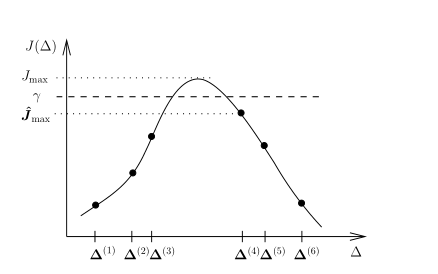
\includegraphics[width=0.49\linewidth]{1.png}
	   \captionof{figure}{MCRA یک طرفه: بدترین عملکرد زمانی که $\hat{J}_{max}<\gamma < J_{max}$}
   \end{center}
   \par  

   MCRA برای عملکرد بدترین حالت متعلق به
   این کلاس است. این الگوریتم شامل محاسبه
   حداکثر تجربی است که با عبارت زیر توصیف میشود:
   \begin{equation*} 	
	   \hat{J}_{max}:= \max_{i=1, 2, ..., N}J(\Delta ^{(i)}) 
   \end{equation*}
   جایی که
   $\Delta (i) \in \mathscr{B} , i=1,2,...,N$
   نمونه های مستقل و یکسان توزیع شده (شناسه) از عدم قطعیت تصادفی هستند.
   ماتریس
   $\Delta$
   با توجه به اندازه گیری احتمال
   $Prob_{\Delta }$
   تولید می شود.
   توجه داشته باشید که حداکثر تجربی
   $\hat{J}_{max}$ 
   خود یک
   متغیر تصادفی است که ارزش آن بستگی به نمونه های تصادفی انتخاب شده
	برای محاسبات دارد.
	شکل. 1 یک طرح از
	$J(\Delta)$
	را نشان می دهد
   و مفهوم این مسئله را بیان میکند.
   \par
   این الگوریتم یک MCRA یک طرفه در زیر است
   برای یک سطح عملکرد داده شده
   $\gamma > 0$
   اگر
   $J_{max}\leq \gamma $
   سپس به وضوح احتمال این که الگوریتم خروجی
   پاسخ صحیح بدهد 1 است.
   از این رو, این الگوریتم همیشه یک راه حل صحیح برای این مثال فراهم می کند.
   از طرف دیگر اگر
   $J_{max}>\gamma $
   سپس احتمال اخذ
   $\hat{J}_{max}\leq\gamma $
   ناصفر است.
   این بدان معنی است که برای این مثال الگوریتم
   می تواند یک نتیجه اشتباه با احتمال غیر صفر بدهد.\par
   اکنون با توجه به اینکه حداکثر تجربی
   $\hat{J}_{max}$
   همیشه کوچکتر است از
   $J_{max}$
   ما باید یک سوال طبیعی مطرح کنیم
   چگونه
   $\hat{J}_{max}$
   به خوبی تخمین حداکثر واقعی می کند؟
   تحت یک
	اندازه نمونه به اندازه کافی بزرگ
   N
   می توان بیانیه احتمالی
   ساخت; به عنوان مثال,\cite{bib22}, \cite{bib23} را ببینید.
   \par   
   کلاس دیگری از MCRA برای مسائل تصمیم گیری این است که از
   الگوریتم های خطای دو طرفه استفاده شود.
   چنین الگوریتم هایی ممکن است یک راه حل اشتباه برای هر دو مورد تولید کنند زمانی که پاسخ بله و خیر است \cite{bib17}.
   مسئله ی میانگین  نمونه ای از یک MCRA  دو طرفه است; برای اطلاعات بیشتر, ما به  \cite{bib24} مراجعه میکنیم.

   \section{الگوریتم های تصادفی لاس وگاس}
   الگوریتم های لاس وگاس و خواص پایه ی آن را معرفی می کنیم.
   این نوع زیاد در زمینه کنترل استفاده نشده است اما برای مسائل اجماع مهم است. 
   
   	\subsection{مقدمات}
	تعریف رسمی در \cite{bib17} به شرح زیر داده شده است:\\
	تعریف 2: الگوریتم های تصادفی لاس وگاس
	الگوریتم های تصادفی هستند که همیشه پاسخ صحیح می دهند
	. تنها تفاوت از یک اجرا به دیگری زمان اجرا است.
	\par
% End Narges's part__________________________________________________________			
% Begin Aaron's part__________________________________________________________
	به دلایل روشنی، به همچین الگوریتم هایی 
	\emph{اشتباه صفر وجهی}
	مونتی کارلو نیز میگویند. به دلیل تصادفی بودن، زمان اجرای الگوریتم نیز رندوم است (مشابه \lr{MCRA}) و ممکن است در هر مرتبه اجرا، زمانی متفاوت داشته باشد. بنابراین، امید ریاضی زمان اجرا مورد توجه است. اشاره کنیم که امید ریاضی با احتساب نمونه های تصادفی ساخته‌شده در هر اجرا است و نه ورودی الگوریتم. بعلاوه، اگر امیدریاضی زمان اجرا، از اردر چندجمله ای باشد، الگوریتم 
	\emph{کارا}
	خوانده می‌شود.
	\par
	یک مثال معروف، الگوریتم کوئیک سورت تصادفی \lr{RQS} است 
	\cite{bib14}, \cite{bib17}
	که در ادامه توضیح داده می‌شود.
	\par
	\textit{مثال ۱} 
	فرض کنید مجموعه 
	\begin{equation*}
		\mathscr{S}_1 = {x_1 , . . . , x_N } 
	\end{equation*}
	از
	$N$
	عدد حقیقی داده شده‌باشد. مسئله مرتب کردن اعداد را در ترتیب افزایشی در نظر بگیرید. الگوریتم \lr{RQS} الگوریتم تصادفی ای است که این مسئله را با یک راه حل که از نظر محاسباتی کارا است حل می‌کند. کلیات الگوریتم بدین صورت است
	\begin{itemize}
		\item[1]
		بصورت تصادفی عدد دلخواه
		$x^{(1)}$
		را از مجموعه
		$\mathscr{S}_1$
		انتخاب می‌کنیم.
		\item[2]
		$x^{(1)}$
		و بقیه اعضای
		$\mathscr{S}_1$
		را مقایسه کنید. مجموعه
		$\mathscr{S}^{(2)}$
		مجموعه اعداد کوچکتر از 
		$x^{(1)}$
		، و مجموعه 
		$\mathscr{S}^{(3)}$
		مجموعه اعداد بزرگتر از
		$x^{(1)}$
		در نظر بگیرید.
		\item[3]
		دو مرحله بالا را به صورت بازگشتی روی مجموعه‌های $\mathscr{S}^{(2)}$ و $\mathscr{S}^{(3)}$ اعمال کنید. نسخه مرتب شده $\mathscr{S}^{(2)}$، $x^{(1)}$، و سپس نسخه مرتب شده $\mathscr{S}^{(3)}$ را خروجی بدهید.
	\end{itemize}
	\par
	منطق تصادفی‌سازی در 1 به شرح زیر است: اگر مجموعه اصلی $\mathscr{S}_1$ به دو مجموعه با کاردینالیتی‌های یکسان تقسیم شود، الگوریتم در کارآمدترین حالت ممکن خواهد بود. با این حال، این به میانه $\mathscr{S}_1$ به عنوان $x^{(1)}$ نیاز دارد که یافتن آن پرهزینه است. انتخاب تصادفی $x^{(1)}$ یک استراتژی ساده است، اما به طور متوسط تخمین خوبی از میانه ارائه می دهد.
	\par
	در یک تحلیل رسمی، زمان اجرا با تعداد مقایسه ها اندازه گیری می شود. نتیجه این است که زمان اجرا مورد انتظار از {$O$($N$log$N$)}\lr است. در واقع، زمان اجرا با احتمال زیاد، یعنی حداقل $1 − 1/N$ از این اردر است.  
	\cite{bib15}
	\textbf{RQS}
	 کارآمدتر از، برای مثال، یک رویکرد بروت-فورس قطعی است که دارای پیچیدگی
	 \lr{$O$($N^2$)} 
	 	است.
	\par
	برای \textbf{RQS}، بدترین حالت زمانی است که عدد به‌طور تصادفی انتخاب شده در $1$ همیشه کوچک‌ترین یا بزرگ‌ترین عدد در مجموعه باشد. سپس، زمان اجرا به اردر \lr{$O$($N^2$)}  می رسد. با این حال، \textbf{RQS} به عنوان یکی از مفیدترین الگوریتم‌های مرتب‌سازی همه‌کاره شناخته می‌شود.
	\cite{bib14}
	$\triangledown$
	\par
	همانطور که در بالا ذکر شد، الگوریتم های لاس وگاس الگوریتم های تصادفی هستند که همیشه نتایج صحیحی را تولید می کنند. واضح است که این ویژگی تنها برای تعداد محدودی از الگوریتم های نوع مونتی کارلو قابل انتظار است. از این رو، کاربرد آنها به طور طبیعی محدود است. یکی از این الگوریتم ها برای مسئله سیستم های سوئیچ شده در \cite{bib11} توسعه داده شده است.
	\par
	\subsection{\lr{LVRA}ها برای مسائل انتخابی غیر قطعی}
	ما اکنون بحثی موازی با بحث سیستم های نامشخص در بخش های 2 و 3 برای الگوریتم های لاس وگاس ارائه می کنیم.
	\par
	ابتدا، به عنوان مجموعه عدم قطعیت، یک زیرمجموعه محدود $\tilde{\mathscr{B}}$ از $\mathscr{B}$ با $N$ عنصر به صورت
	\begin{equation*}
		\tilde{\mathscr{B}} = \left\{\tilde{\Delta}_1, \tilde{\Delta}_2, ..., \tilde{\Delta}_N\right\} \subset \mathscr{B}
	\end{equation*}
	را در نظر می‌گیریم.

	\begin{center}
		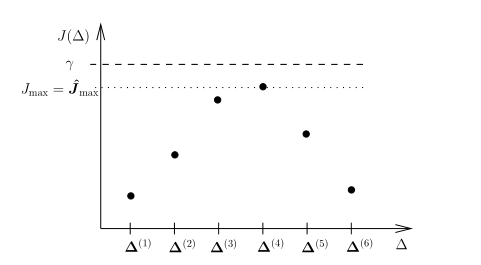
\includegraphics[width=0.35\linewidth]{2.png}
		\captionof{figure}{\lr{:LVRA} بدترین عملکرد وقتی $J_{max}=\widehat{J} < \gamma$}
	\end{center}

	با فرض اینکه ماتریس های نامشخص در $\tilde{\mathscr{B}}$ متغیرهای تصادفی هستند، یک اندازه گیری احتمال گسسته را در نظر می گیریم؛ دقیقا همانند بخش II، این اندازه گیری با Prob$_\Delta$ نشان داده می شود. به طور مشابه، فرض کنید تابع عملکرد $J : \tilde{\mathscr{B}} → \mathbb{R}$ باشد. مسئله تحلیل استحکام کلی این است که ببینیم آیا برای یک سطح عملکرد معین $\gamma > 0$، $J(\Delta) \leq \gamma$ برای همه $\Delta \in \tilde{\mathscr{B}}$ است یا خیر. بدترین حالت مربوطه بصورت
	
	\begin{equation}
		J_{max} := \max_{\Delta \in \tilde{\mathscr{B}}}J(\Delta)
	\end{equation}
	است، و حالت میانگین بصورت
	\begin{equation*}
		J_{ave} := E_\Delta\left[J(\Delta)\right] = \sum_{i=1}^N J(\tilde{\Delta}_i)Prob_\Delta(\tilde{\Delta}_i)
	\end{equation*}
	است.
	ما اکنون مسئله انتخابی غیرقطعی را برای عملکرد بدترین حالت در نظر می گیریم. با فرض یک اسکالر $\gamma > 0$، بررسی کنید که آیا 
	$J_max \leq \gamma$
	برقرار است یا خیر.
	\lr{LVRA}
	 برای این مورد به شرح زیر است: فرض کنید $\tilde{\mathscr{B}}_0 = \tilde{\mathscr{B}}$ و فرض کنید $k = 1$. همچنین، فرض کنید $\bar{J}^{(0)} = -\inf$. در مرحله $k$th، به طور تصادفی یک نمونه $\Delta^{(k)}$ از $\tilde{\mathscr{B}}_{k-1}$ انتخاب کنید. سپس، قرار دهید 
	$\bar{J}^{(k)} = max \left\{J(\Delta^{(k)}), \bar{J}^{(k-1)}\right\}$
	 و $\tilde{\mathscr{B}}_k = \tilde{\mathscr{B}}_{k-1} \ {\Delta^{(k)}}$، و به مرحله بعد بروید. پس از مرحله $N$ام، حداکثر عملکرد نسبت به نمونه ها توسط $\hat{J}_{max} = \bar{J}^{(N)}$ محاسبه می‌شود.
	\par
	این الگوریتم همیشه پاسخ صحیح را خروجی می دهد و از این رو از نوع لاس وگاس است. برای مثال $(J_{max} \leq \gamma$ یا مثال $J_{max} > \gamma)$، مقدار \textbf{$\hat{J}_{max}$} که الگوریتم تولید می‌کند با مقدار واقعی $J_{max}$ منطبق می‌شود. این موضوع در شکل 2 نشان داده شده است.
	\par
	وقتی $N$ بزرگ است، پیچیدگی محاسباتی را می توان با اصلاح الگوریتمی که توضیح دادیم کاهش داد. الگوریتم به دست آمده از نوع مونتی کارلو است. این را می توان با توقف در مرحله $k$ام با $k <N$ و با محاسبه حداکثر عملکرد روی نمونه $k$ انجام داد. در واقع الگوریتم حاصل به یک \lr{MCRA} یک طرفه تبدیل می شود. ما خاطرنشان می کنیم که این رویکرد ارتباط نزدیکی با بهینه سازی ترتیبی دارد. به عنوان مثال، \cite{bib08} را ببینید. هدف در آنجا یافتن حداکثر مقدار عملکرد نیست، بلکه مقداری است که حداقل در $m$ تا بزرگترین باشد.
	\par
	عملکرد متوسط مورد نیز می تواند به طور مشابهی بررسی شود.			
	
	\section{الگوریتم های تصادفی لاس وگاس برای اجماع متوسط توزیع شده}
	در این بخش، چندین مسئله در اجماع میانگین توزیع شده ارائه می‌کنیم که در آن کاربرد الگوریتم‌های نوع لاس وگاس می‌تواند مؤثر و گاهی اوقات در واقع حیاتی باشد.
	
	\subsection{\textit{حالت مسئله عمومی}}
	شبکه‌ای از $N$ گره را در نظر بگیرید که گراف ($\mathscr{V}$, $\mathscr{E}$) می‌نامیم، که در آن $\mathscr{V} := {1, 2, . . . , N }$ مجموعه گره ها و $\mathscr{E}$ مجموعه یال ها است. فرض می‌شود که گراف بدون جهت و همبند است (به‌عنوان مثال، \cite{bib17} را برای مقدمه‌ای بر نظریه گراف‌های تصادفی ببینید). این بدان معنی است که یال ها با جهت علامت گذاری نشده اند و برای هر $i، j \in \mathscr{V}$، مسیری وجود دارد که گره های $i$ و $j$ را به هم متصل می کند. در زمان $k$، هر گره $i$ دارای یک مقدار اسکالر $x_i(k)$ است که مقدار اولیه آن $x_i(0)$ است.
	\par
	هدف ارائه الگوریتمی است که (I) گره ها مقادیر $x_i(k)$ خود را با استفاده از اطلاعات ارسالی از همسایگان خود به روز کنند و (II) مقادیر گره ها در نهایت به میانگین مقادیر اولیه همگرا شوند. برای این منظور، برای یک الگوریتم اجماع، دو عنصر وجود دارد که باید تعیین شود: قوانینی برای به‌روزرسانی مقادیر گره ها و همسایه هایی که هر گره باید با آنها ارتباط برقرار کند.
	\par
	این مسئله نسخه خاصی از اجماع توزیع شده است. به طور کلی، مسائل اجماع دنبال این نیستند که مقادیر گره ها به کدام عدد باید همگرا شوند، بلکه فقط باید مقدار آنها برای همه گره ها یکسان باشد. در ادامه به سه حالت از این مسئله می پردازیم. تفاوت در محدوده مقادیر گره‌ها است: اعداد واقعی، اعداد صحیح (کوانتیزه شده) و اعداد باینری.
	\par
	ابتدا برخی نماد را که در سراسر این بخش مورد استفاده قرار خواهند گرفت، معرفی می کنیم. فرض کنید بردار $N$-بعدی متشکل از همه مقادیر گره در زمان 
	$k$ 
	$x(k) = [x_1(k) \hdots x_N(k)]^T$
	 باشد. الگوی ارتباطی برای گره‌ها در زمان
	$k$
	 توسط مجموعه یال
	$\tilde{\mathscr{E}}(k) \subset \mathscr{E}$
	 مشخص می‌شود، یعنی اگر 
	$\{i, j\} \in \tilde{\mathscr{E}}$
	 ، سپس
	$x_i(k)$
	 با استفاده از 
	$x_j(k)$
	 به روز می شود و بالعکس. در این حالت، گره‌های $i$ و $j$ در این زمان \emph{همسایگان} یکدیگر هستند. به طور کلی، همسایگان یک گره ممکن است در طول زمان تغییر کنند.
	\subsection{\textit{حالت مقدار حقیقی}}
	ما ابتدا حالتی را ارائه می کنیم که مقادیر گره‌ها اعداد حقیقی اند؛ که در \cite{bib28} مطالعه شده است. می گوییم اجماع متوسط (به معنای قطعی) در صورتی حاصل می شود که شرط زیر برآورده شود:
	\begin{equation}
		\lim_{k \rightarrow \inf} x_i(k) = \frac{1}{N} \sum_{j=1}^{N} x_j(0) \text{ for all } i = 1, ..., N.
	\end{equation}
	قانون به‌روزرسانی برای گره $i$ یک فرم خطی به شکل
	\begin{equation}
		x_i(k+1)=W_{ii}(k) x_i(k) + \sum_{j \in \mathscr{N}_i(k)} W_{ij}(k) x_j(k),
	\end{equation}
	می‌گیرد؛ که
	$\mathscr{N}_i(k) := \{j : \{i، j\} \in \tilde{\mathscr{E}}(k)\}$
	مجموعه ی همسایگان برای گره $i$ در زمان $k$، و $W_{ij}(k)$ وزن هستند. وزن ها در زمان تغییر می کنند و بر اساس
	\begin{equation}
		W_{ij}(k)=\begin{cases}
			\frac{1}{1+max\{d_{i}(k),d_{j}(k)\}} & \text{if }\{i,j\}\in \ensuremath{\tilde{\mathscr{E}}(k),}\\
			1-\sum_{l\in\mathscr{N}_{i}(k)}W_{il}(k) & \text{if }i=j\\
			0 & \text{otherwise,}
		\end{cases}
	\end{equation}
	مشخص می‌شوند؛ که در آن $d_i(k)$ نشان دهنده کاردینالیتی $\mathscr{N}_i(k)$، یعنی تعداد همسایگان برای گره $i$ است. توجه داشته باشید که مجموع وزن‌ها در هر گره یک است. این باعث می شود ماتریس $W$ یک ماتریس تصادفی باشد. در \cite{bib28}، اشاره شده است که وزن‌های $Wij(k)$ در (6) از الگوریتم متروپلیس استفاده شده در زنجیره مارکوف مونتی کارلو اتخاذ شده‌اند.
	\par
	قانون به روز رسانی در (5) را می توان به صورت توزیع شده و علّی اجرا کرد. این به این دلیل است که گره ها فقط به دانستن مقادیر رسیده از همسایگان خود در زمان به روز رسانی نیاز دارند. در مورد الگوی ارتباطی مشخص شده توسط $\tilde{\mathscr{E}}(k)$, $k \in \mathbb{Z}_+$، فرض به شرح زیر است: گراف ($\mathscr{V}$ , $\bigcup_{s \geq k} \tilde{\mathscr{E}}(s)$) یک گراف همبند برای هر $k$ است. به عبارتی، یعنی مجموع‌ مجموعه‌های یال هایی که در طول زمان بی‌نهایت مرتبه رخ می‌دهند، آن را به یک گراف همبند تبدیل می‌کند.
	\par
	آنچه در زیر آمده است،‌ نتیجه اصلی \cite{bib28} است.
	\par
	\textit{قضیه 1:}
	تحت قانون به‌روزرسانی در (5) و الگوی ارتباطی خاصی که شرایط اینکه گراف ($\mathscr{V}$, $\bigcup_{s \geq k} \tilde{\mathscr{E}}(s)$) یک گراف همبند برای همه $k$ است را ارضا می‌کند، اجماع میانگین توزیع شده با تعریف (4) برای هر شرط اولیه $x(0) \in \mathbb{R}^N$ بدست می‌آید.
	\par
	این قضیه شرطی را در $\tilde{\mathscr{E}}(k)$ ارائه می‌کند که باید در زمان پیاده سازی برای اجماع متوسط به معنای قطعی مشخص شود. شرایط مشابهی در طرح‌های دیگر به‌کار می‌رود، به‌عنوان مثال، \cite{bib05}، \cite{bib12} و  \cite{bib16}.
	\par
	یک راه ساده برای پیاده سازی یک الگوی ارتباطی با ویژگی مورد نظر، استفاده از تصادفی سازی است: هر گره $i$ با یک همسایه به طور تصادفی و مستقل انتخاب شده $j_k$ ارتباط برقرار می کند که $\{i, j_k\} \in \mathscr{E}$ را در زمان $k$ برآورده می کند. به طور خاص، احتمالی مثبت به هر یال $\{i, j\}$ در $\mathscr{E}$ اختصاص می‌دهیم. از آنجایی که ($\mathscr{V}$, $\mathscr{E}$) یک گراف همبند است، شرط در الگوی ارتباطی به طور احتمالی برقرار است. یعنی به ازای هر $k$، احتمال اینکه نمودار ($\mathscr{V}$, $\bigcup_{s \geq k} \tilde{\mathscr{E}}(s)$) همبند شود یک است. از این رو، الگوریتم حاصل به اجماع متوسط در (4) با احتمال یک برای هر $x(0)$ دست می یابد.
	\par
	یک طرح اجماع میانگین تصادفی دیگر نیز در \cite{bib10} پیشنهاد شده است، که در آن یال های گراف به طور تصادفی و مستقل از یکدیگر انتخاب می‌شوند. این مقاله یک تحلیل احتمالی از همگرایی ارائه می دهد. این طرح بر اساس یک پروتکل ارتباطی داده‌های نمونه‌برداری شده است و وزن‌هایی را به کار می‌گیرد که با موارد (6) متفاوت است. سایر آثاری که از الگوهای ارتباطی تصادفی‌ سازی شده استفاده می‌کنند عبارتند از: \cite{bib07}، \cite{bib21} و  \cite{bib27}.

% End Aaron's part__________________________________________________________			
% Begin Fateme's part__________________________________________________________

			\subsection{\textit{حالت مقدار کوانتیزه شده}}
			
			این طرح در 
			 \cite{bib13}
			 پیشنهاد شده است.
			 اینجا منظور از کوانتیزه شدن، این است که مقادیر گره‌ها اعداد صحیح هستند. این مسئله‌ی اجماع، نیازمند چاره‌ای متفاوت از حالت مقدار حقیقی است. برای شروع، میانگین از مقادیر اولیه ممکن است یک عدد صحیح نباشند. بنابراین، مقدار مورد نظر یک تقریب عدد صحیح از میانگین واقعی است و لزوما منحصر به فرد نیست. علاوه بر این، می توان در زمان محدود به اجماع رسید زیرا گره ها در اعداد صحیح در هر لحظه به‌روز می شوند.
			 
			 به طور خاص تر، اگر شرایط زیر برقرار باشند، گفته می‌شود الگوریتم به متوسط اجماع کوانتیزه‌شده می‌رسد:
			 
			\begin{enumerate}
				\item همیشه مقادیر اعداد صحیح هستند:
				 $x_{i}(k)\in \mathbb{Z}, \; \forall{i, k}$.
				\item مجموع مقادیر گره‌ها ثابت می‌ماند:
				$\sum_{i=1}^{N}x_{i}(k)=\sum_{i=1}^{N}x_{i}(0)$ 
				برای هر 
				$k$.
				\item همه‌ی مقادیر به میانگین کوانتیزه شده همگرا می‌شوند: 
				 $k^{*}$ 
				وجود دارد که 
				$x_{i}(k)\in \left\{ \overline{x}, \overline{x}+1 \right\}$ 
				برای هر 
				$k > k^{*}$ 
				و 
				$i$، 
				که 
				$\overline{x}=\left\lfloor \sum_{i=1}^{N}x_{i}(0)/N \right\rfloor$.
			\end{enumerate}
		
		\begin{center}
			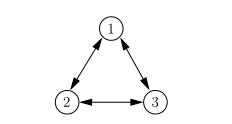
\includegraphics[width=0.35\linewidth]{3.png}
			\captionof{figure}{گرافی با 3 گره}
		\end{center}
			
			در
			 \cite{bib13}
			 یک کلاس از الگوریتم‌های تصادفی به نام
			 \textit{الگوریتم‌های گاسیپ کوانتیزه‌شده} 
			 پیشنهاد شده است؛
			  \cite{bib06} 
			 را نیز ببینید.
			  
			  موارد زیر، ملزومات چنین الگوریتم‌هایی هستند: در زمان 
			  $k$
			  یک یال 
			  $\left\{ i, j \right\} \in \varepsilon$ 
			  به روش
			  \lr{i.i.d.}
			  به طور تصادفی انتخاب می‌شود.
			  فرض کنید 
			$D_{ij}(k)=\left| x_{i}(k)-x_{j}(k) \right|$.
			
			\begin{enumerate}
				\item اگر
				$D_{ij}(k)=0$، 
				آنگاه مقدار گره‌های 
				$i$ 
				و 
				$j$ 
				در زمان 
				$k+1$ 
				یکسان باقی می‌مانند. 
				
				\item اگر
				$D_{ij}(k)=1$، 
				آنگاه مقادیر مطابق زیر جابجا می‌شوند:
				\begin{equation}
					x_{i}(k+1)=x_(j)(k) \text{ و } x_{j}(k+1)=x_{i}(k).
				\end{equation}
				
				\item در غیر این صورت، بروزرسانی مقادیر به صورت زیر است:
				\begin{equation*}
					x_{i}(k+1)+x_{j}(k+1)=x_{i}(k)+x_{j}(k),
				\end{equation*}
				\begin{equation*}
					D_{ij}(k+1)< D_{ij}(k).
				\end{equation*}
			\end{enumerate}
		
		توجه کنید که الگوریتم‌ها در این کلاس با توجه به تعریف، رندوم هستند. یکی از راه های تعیین توزیع برای انتخاب گره‌ها، تخصیص احتمالات مثبت به همه‌ی گره‌ها در گراف است. ما خوانندگان را به 
		\cite{bib13} 
		برای چند مورد از الگوریتم‌های صریح گاسیپ کوانتیزه شده که ملزومات فوق را ارضا میکنند، ارجاع می‌هیم. همچنین تاکید می‌کنیم که این الگوریتم‌ها با الگوریتم‌های بخش 
		\lr{V-B} 
		متفاوت هستند.
		
		\textit{\textbf{قضیه 2:}}
		برای هر شرابط اولیه‌ی 
		$x(0)\in \mathbb{Z}^{\mathrm{N}}$، 
		یک الگوریتم گاسیپ کوانتیزه شده با احتمال یک، به یک اجماع متوسط کوانتیزه شده در تعدادی گام متناهی می‌رسد.
		
		یکی از جنبه های جالب این الگوریتم، تصادفی سازی ضروری است. این می‌تواند با یک مثال که در 
		\cite{bib13} 
		آمده، تصویرسازی شود. 
		یک گراف با سه گره مانند شکل 3 در نظر بگیرید. در ابتدا، گره 
		$i$ 
		مقادیر 
		$i = 1, 2, 3$ 
		را می‌گیرد و بنابراین، مقدار میانگین برابر $2$ می‌شود.
		فرض کنید ما یک طرح قطعی دوره‌ای برای انتخاب یال با دوره‌ی تناوب 
		$3$ 
		به صورت 
		$\left\{ 1, 2 \right\}, \left\{ 1, 3 \right\}, \left\{ 3, 2 \right\}, \left\{ 1, 2 \right\}, \ldots$ 
		به کار بگیریم. طبق این طرح، واضح است که فقط جابجایی در (7) همیشه اتفاق می‌افتد. بنابراین، مجموعه‌ی مقادیر گره‌ها 
		$1$، 
		$2$ 
		و
		$3$ 
		باقی می‌ماند و هرگز به مقادیر اجماع نمی‌رسد. در مقابل، با انتخاب تصادفی گره‌ها، میانگین اجماع در چند مرحله امکان پذیر است.
		
		در 
		\cite{bib13} 
		تحلیل‌های احتمالی بیشتری درباره‌ی زمان اجرای مورد انتظار برای رسیدن به اجماع کوانتیزه شده آورده شده‌اند. به طور خاص، اگر گراف همبند کامل یا خطی باشد، آنگاه زمان اجرای مورد انتظار، چند جمله‌ای برجسب تعداد گره‌ها است. بنابراین این الگوریتم یک مثال از یک الگوریتم لاس وگاس است. این، با حالت مقدار حقیقی در بخش 
		\lr{V-B} 
		در تقابل است.
		
		\subsection{\textit{حالت مقدار دودویی}}
		
		سومین مسئله‌ی اجماع زمانیست که عوامل، مقادیر باینری 
		$x_{i}(k) \in \left\{ 0,1 \right\}$ 
		برای هر 
		$i$ 
		و 
		$k$ 
		را اتخاذ می‌کنند. به طور خاص، مسئله‌ای که در اینجا به آن می‌پردازیم، با عنوان 
		\lr{\textit{Byzantine agreement}} 
		شناخته می‌شود 
		\cite{bib17}. 
		ما نشان خواهیم داد که در این حالت، نتایج قوی‌تری به نفع طرح‌های تصادفی قابل دسترسی هستند.
	
	یک ویژگی متمایزکننده‌ی این مسئله این است که بعضی از عوامل 
	$N$ 
	معیوب هستند. این عوامل، ممکن است عوامل نامعیوب را فریب دهند و حتی ممکن است که مخفیانه باهم ارتباط داشته باشند. ما فرض می‌کنیم به تعداد 
	$N_{f}$ 
از این عوامل داریم که ثابت اند اما هویت آنها برای عوامل نامعیوب ناشناخته است. با توجه به الگوی ارتباطی، گراف همبند کامل است. هر عامل در زمان 
$k$ 
پیامی را به تمام عوامل دیگر می‌فرستد؛ عوامل معیوب، ممکن است پیام‌های متفاوتی به سایرین بفرستند. درنتیجه، تصادفی سازی در الگوی ارتباطی رخ نمی‌هد. در عوض، یک پرتاب سکه توسط یک طرف قابل اعتماد که نتیجه را برای تمام عوامل در هر 
$k$ 
می‌فرستد، انجام می‌شود.

هدف، دستیابی به نوعی اجماع متوسط حتی در بدترین حالت ​​است. اگر هر عامل 
$i$ 
مقدار  تصمیم 
$y_{i} \in \left\{ 0,1 \right\}$ 
را به صورت زیر تعیین کند، می‌گوییم 
\textit{اجماع دودویی} 
حاصل شده است:
\begin{enumerate}
	\item همه‌ی عوامل نامعیوب به یک مقدار تصمیم برسند؛
	\item اگر تمام عوامل نامعیوب مقدار اولیه‌ی یکسان 
	$x_{i}(0)$ 
	را داشته باشند، آنگاه 
	$y_{i} = x_{i}(0)$.
\end{enumerate}
حالت ساده‌ای را در نظر می‌گیریم که در آن 
$N$ 
مضربی از $8$ است و 
$N_{f} < N/8$. 
همچنین قرار می‌هیم:
\begin{equation*}
	L:=5N/8+1,\; H:=3N/4+1,\; G:=7N/8.
\end{equation*}

الگوریتمی که برای هر عامل $i$ ارائه می‌دهیم، براساس 
\cite{bib19} 
است؛ اساسا، عامل مورد نظر مقدار خودش را می‌فرستد و با توجه به اکثریت مقادیری که دریافت کرده، تصمیم می‌گیرد.

\begin{center}
	\begin{tabular}{||c||} 
		\hline
		1) \, ارسال مقدار 
		$x_{i}(k)$ 
		به عوامل دیگر و دریافت \\
		$x_{j}(k), \; j\neq i$ 
		از آنها در زمان 
		$k$.\\ [0.5ex] 
		\hline
		2) \, تنظیم 
		\textit{مقدار اکثریت} 
		$m_{i}(k)\in \left\{ 0,1 \right\}$ 
		به چیزی که \\
		اکثر عوامل آن را به عنوان مقدار خود فرستاده اند. سپس،\\
		 قرار دادن مقدار
		\textit{شمارش} 
		$t_{i}(k)$ 
		برابر با تعداد عواملی که مقادیرشان برابر 
		$m_{i}(k)$ 
		است.\\ 
		\hline
		3) \, حال، با توجه به نتیجه‌ی پرتاب سکه، مقدار 
		\textit{آستانه} 
		$\overline{t}(k)$ \\
		را برابر 
		$L$ 
		قرار دهید اگر سکه شیر بیاید؛\\
		 و درغیراینصورت، مقدار آن را 
		$H$ 
		بگذارید.\\
		\hline
		4) \, تنظیم مقدار 
		$x_{i}(k)$ 
		به مقدار اکثریت 
		$m_{i}(k)$ \\
		اگر  
		$t_{i}(k) \ge \overline{t}(k)$ 
		و در غیر اینصورت به $0$.\\
		\hline
		5) \, اگر 
		$t_{i}(k) \ge G$، 
		آنگاه مقدار تصمیم را برابر 
		$y_{i}$ \\
		را برابر 
		$m_{i}(k)$ 
		قرار دهید.\\
		\hline
	\end{tabular}
\end{center}


دو راه حل ساده وجود دارد. (الف) زمانیکه همه‌ی عوامل نامعیوب در یک نقطه مقدار مشترک دارند، همه‌ی آنها در تعدادی گام ثابت، این مقدار را به عنوان مقدار تصمیم خود اتخاذ می‌کنند. (ب) وقتی دو عامل نامعیوب دو مقدار اکثریت متفاوت دارند، آنگاه همه‌ی مقادیر 
$x_{i}(k)$ 
در این گام صفر می‌شوند زیرا هیچ یک از شمارش ها از آستانه عبور نکرده اند.

حالت جالب زمانیست که همه‌ی عوامل نامعیوب مقدار اکثریت یکسانی دارند. آنگاه، عوامل معیوب این شانس را دارند که آنها را سردرگم کنند. این کار می‌تواند با ساخت چند عامل نامعیوب که شمارش برخی از آنها از آستانه عبور می‌کند و شمارش سایرین، از آستانه کمتر است انجام شود.
با این حال، طبق این طرح، شانس محدود است. چون 
$H−L \ge N_{f}$، 
عوامل معیوب می‌توانند هر عامل را فقط برای یکی از آستانه های 
$L$ 
یا 
$H$ 
فریب دهند. 
علاوه بر این، آستانه به طور رندوم بین 
$L$ 
و 
$H$ 
به علت پرتاب سکه تغییر می‌کند. در نتیجه، احتمال فریب 
$1/2$ 
است. از سوی دیگر، زمانی که آنها نمی توانند فریب دهند، همه عوامل غیر معیوب ارزش یکسانی دارند، که منجر به اجماع می شود.

نتیجه اصلی در مورد 
\lr{Byzantine agreement problem} 
در زیر آورده شده است 
\cite{bib17}.

\textit{\textbf{قضیه 3:}} برای الگوریتمی که در بالا توصیف شد، اجماع دودویی با احتمال یک برای هر مقدار اولیه‌ی 
$x(0) \in \left\{ 0,1 \right\}^{N}$ 
به دست می‌آید. همچنین، تعداد گام‌های مورد نیاز، ثابت است.

این قضیه مطرح می‌کند که الگوریتم اجماع، یک نوع موثر از الگوریتم لاس وگاس است. در مقابل، واضح است که هر الگوریتم قطعی نیازمند 
$N_{f}+1$ 
گام است 
\cite{bib17}. 
تاکید شده است که نتایج قوی‌تری نیز در حوزه‌ی محاسبات توزیع شده بدست آمده است. یکی از آنها 
\textit{نتیجه‌ی ناممکن} 
برای یک ورژن ناهماهنگ از مسئله‌ی اجماع دودویی است 
\cite{bib09}.
 این نتیجه بیان می‌کند که اگر هیچ ساعت هماهنگی متعلق به عوامل وجود نداشته باشد و اگر هیچ فرضی از نمونه برداری دوره ها از عوامل وجود نداشته باشد، برای هر الگوریتم قطعی، رسیدن به اجماع ناممکن است. طرح های تصادفی مثل پرتاب سکه در این حالت به خوبی نشان داده شده‌اند. برای بررسی
 این موضوع، که همچنین شامل بسیاری از پیشرفت های اخیر در الگوریتم اصلی است، به 
 \cite{bib02} 
اشاره می‌کنیم.


	\section{نتیجه‌گیری}
	
	در این مقاله، درباره‌ی چند واریانت از مسئله‌ی اجماع متوسط و نقش الگوریتم‌های احتمالی در این زمینه، بحث کردیم. همچنبن، نشان داده شد که کلاس الگوریتم‌های تصادفی لاس وگاس، که اخیرا در حوزه‌ی سیستم‌ها و کنترل به کار گرفته شده‌اند
	\cite{bib11}، 
	\cite{bib24}، 
	موثر و گاهی حیاتی است.
% End Fateme's part__________________________________________________________
	
	\begin{thebibliography}{30}
		\bibitem{bib01} P. J. Antsaklis and J. Baillieul, Guest Editors. Special Issue on the Technology of Networked Control Systems.\textit{Proc. IEEE,} 95(1), 2007.
		
		
		\bibitem{bib02} J. Aspnes. Randomized protocols for asynchronous consensus. \textit{Distributed Computing}, 16:165–175, 2003.
		
		
		\bibitem{bib03} D. P. Bertsekas and J. N. Tsitsiklis.\textit{Parallel and Distributed Computation: Numerical Methods.} Prentice-Hall, Englewood Cliffs, NJ,1989.
		
		
		\bibitem{bib04} D. P. Bertsekas and J. N. Tsitsiklis. Comments on “Coordination of groups of mobile autonomous agents using nearest neighbor rules”. \textit{IEEE Trans. Autom. Control,} 52:968–969, 2007.
		
		
		\bibitem{bib05} V. D. Blondel, J. M. Hendrickx, A. Olshevsky, and J. N. Tsitsiklis. Convergence in multiagent coordination, consensus, and flocking. In \textit{Proc. 44th IEEE Conf. on Decision and Control and European Control Conf.,} pages 2996–3000, 2005.
		
		
		\bibitem{bib06} S. Boyd, A. Ghosh, B. Prabhakar, and D. Shah. Randomized gossip algorithms. \textit{IEEE Trans. Information Theory}, 52:2508–2530, 2006.
		
		
		\bibitem{bib07} R. Carli, F. Fagnani, M. Focoso, A. Speranzon, and S. Zampieri. Communication constraints in the average consensus problem. \textit{Automatica,} 44:671–684, 2008.
		
		
		\bibitem{bib08} M. Deng and Y.-C. Ho. An ordinal optimization approach to optimal control problems. \textit{ Automatica,} 35:331–338, 1999.
		
		
		\bibitem{bib09} M. J. Fisher, N. A. Lynch, and M. S. Paterson. Impossibility of distributed consensus with one faulty processor. \textit{J. ACM}, 32:374–382, 1985.
		
		
		\bibitem{bib10} Y. Hatano and M. Mesbahi. Agreement over random networks. \textit{IEEE Trans. Autom. Control,} 50:1867–72, 2005.
		
		
		\bibitem{bib11} H. Ishii and R. Tempo. Probabilistic sorting and stabilization of switched systems. Submitted for publication, 2007.
		
		
		\bibitem{bib12} A. Jadbabaie, J. Lin, and A. S. Morse. Coordination of groups of mobile autonomous agents using nearest neighbor rules. \textit{IEEE Trans. Autom. Control}, 48:988–1001, 2003.
		
		
		\bibitem{bib13} A. Kashyap, T. Bas¸ar, and R. Srikant. Quantized consensus. \textit{Automatica}, 43:1192–1203, 2007.
		
		
		\bibitem{bib14} D. E. Knuth. \textit{The Art of Computer Programming,} 2nd edition, volume 3: Sorting and Searching. Addison-Wesley, Reading, MA, 1998.
		
		
		\bibitem{bib15} M. Mitzenmacher and E. Upfal. \textit{Probability and Computing: Randomized Algorithms and Probabilistic Analysis.} Cambridge University Press, 2005.
		
		
		\bibitem{bib16} L. Moreau.Stability of multiagent systems with time-dependent communication links.\textit{IEEE Trans. Autom. Control}, 50:169–182,2005.
		
		
		\bibitem{bib17} R. Motwani and P. Raghavan. \textit{Randomized Algorithms}. Cambridge University Press, 1995.
		
		
		\bibitem{bib18} R. Olfati-Saber and R. Murray. Consensus problems in networks of agents with switching topology and time-delays. \textit{IEEE Trans. Autom. Control,} 49:1520–1533, 2004.
		
		
		\bibitem{bib19} M. O. Rabin. Randomized Byzantin generals. In \textit{Proc. Annual Symp. on Foundations of Computer Science}, pages 403–409, 1983.
		
		
		\bibitem{bib20} A. V. Savkin. Coordinated collective motion of groups of autonomous robots: Analysis of Vicsek’s model. \textit{IEEE Trans. Autom. Control,}49:981–983, 2004.
		
		
		\bibitem{bib21} A. Tahbaz-Salehi and A. Jadbabaie. Necessary and sufficient conditions for consensus over random independent and identically distributed switching graphs. In \textit{Proc. 46th IEEE Conf. on Decision and Control,} pages 4209–4214, 2007.
		
		
		\bibitem{bib22} R. Tempo, E. W. Bai, and F. Dabbene. Probabilistic robustness analysis: Explicit bounds for the minimum number of samples. \textit{Systems and Control Letters}, 30:237–242, 1997.
		
		
		\bibitem{bib23}  R. Tempo, G. Calafiore, and F. Dabbene. \textit{Randomized Algorithms for Analysis and Control of Uncertain Systems.} Springer, London, 2005.
		
		
		\bibitem{bib24} R. Tempo and H. Ishii. Monte Carlo and Las Vegas randomized algorithms for systems and control: An introduction. European J. Control, 13:189–203, 2007.
		
		
		\bibitem{bib25} J. N. Tsitsiklis. \textit{Problems in Decentralized Decision Making and Computation}. PhD thesis, Dept. of Electrical Engineering and Computer Science, MIT, 1984. \href{http://web.mit.edu/jnt/www/Papers/PhD-84-jnt.pdf.}{http://web.mit.edu/jnt/www/Papers/PhD-84-jnt.pdf.}
		
		
		\bibitem{bib26} M. Vidyasagar. Statistical learning theory and randomized algorithms for control. \textit{IEEE Control Systems Magazine,} 18(6):69–85, 1998
		
		
		\bibitem{bib27} C. W. Wu. Synchronization and convergence of linear dynamics in random directed networks. \textit{IEEE Trans. Autom. Control,} 51:1207–1210, 2006.
		
		
		\bibitem{bib28} L. Xiao, S. Boyd, and S. Lall. A scheme for robust distributed sensor fusion based on average consensus. In \textit{Proc. Conf. on Information Processing in Sensor Networks,} pages 63–70, 2005.
	\end{thebibliography}

\end{document}